\documentclass[10pt]{article}

%%%%%%%%%%%%%%%%%%%%%%%%%%%%%%%%%%%%%%%%%%%%%%%%%%%%%%%%%%%%%%%%%%%%%%%%%%%%%%%%%%%%%%%%%%%%%%%%%%%%%%%%%%%%%%%%%%%%%
%%                                              LOAD PACKAGES
%%%%%%%%%%%%%%%%%%%%%%%%%%%%%%%%%%%%%%%%%%%%%%%%%%%%%%%%%%%%%%%%%%%%%%%%%%%%%%%%%%%%%%%%%%%%%%%%%%%%%%%%%%%%%%%%%%%%%
\usepackage{ifpdf}
\usepackage[load-configurations=abbreviations]{siunitx}     % define units
\usepackage{color}                                          % add colors to text (and highlight)
\usepackage{soul}                                           % for highlighting
\usepackage{amsmath}                                        % for mathematical formula
\usepackage{amssymb}                                        % mathematical symbols (might not be useful)
\usepackage{booktabs}                                       % for arrays: toprule, midrule, bottomrule
\usepackage{multirow}                                       % for arrays
\usepackage{graphicx}                                       % for \includegraphics
\usepackage{rotating}                                       % for sideways and other rotating stuffs
\usepackage{authblk}                                        % for authors and affiliations
\usepackage[printonlyused,withpage]{acronym}
%\usepackage[printonlyused,withpage,nohyperlinks]{acronym}


\ifpdf
    \usepackage[subrefformat=parens]{subcaption}                % for subfigures (replaces the subfig package:
                                                                % more up-to-date and works well with hyperref)
    \pdfoptionpdfminorversion=6                                 % Solves "found PDF version 1.6, but at most version
                                                                % 1.5 allowed" warning
\fi

\usepackage[
            backend         = biber
            , style         = authoryear-comp   %numeric-comp, authoryear-comp
            , sorting       = nyt               % name, title, year
            , maxbibnames   = 10                % maximum number of authors to mention in the bibliography, if reached,
            , minbibnames   = 1                 % the number of authors to cite is set to minbibnames (et al.)
            , maxcitenames  = 2                 % same for within the text (makes sense with only specific cite styles)
            , mincitenames  = 1
            , backref       = false             % indicate or not the page on which the bibliography item is cited
            , backrefstyle  = three
            , abbreviate    = true              % default (Volume -> Vol., pages -> pp., ...)
            , doi           = false
            , isbn          = false
            , url           = false
            , eprint        = false
            , firstinits    = true              % all first and middle names as initials
            , uniquename    = init              % Disambiguate names using initials only (to be compatible with firstinits = true)
            ]{biblatex}

%\addbibresource{d:/KULeuven/PhD/MendeleyBiblioAbbr.bib}
%\addbibresource{d:/KULeuven/PhD/Publish/JournalPublications/Neuroimage/draft/AdditionalBiblioAbbr.bib}
\addbibresource{d:/KULeuven/PhD/MendeleyBiblio.bib}
%\addbibresource{d:/KULeuven/PhD/Publish/JournalPublications/Neuroimage/draft/AdditionalBiblio.bib}

% TO LOAD LAST FOR COMMANDS NOT TO BE OVERWRITTEN
\usepackage[bookmarksopen,colorlinks,linkcolor=blue,citecolor=blue]{hyperref} % for \autoref and hyperlinks

%%%%%%%%%%%%%%%%%%%%%%%%%%%%%%%%%%%%%%%%%%%%%%%%%%%%%%%%%%%%%%%%%%%%%%%%%%%%%%%%%%%%%%%%%%%%%%%%%%%%%%%%%%%%%%%%%%%%%
%%                                           DOCUMENT OPTIONS
%%%%%%%%%%%%%%%%%%%%%%%%%%%%%%%%%%%%%%%%%%%%%%%%%%%%%%%%%%%%%%%%%%%%%%%%%%%%%%%%%%%%%%%%%%%%%%%%%%%%%%%%%%%%%%%%%%%%%

%--------------------------------------------------
% biblatex options
%--------------------------------------------------

%% remove "in:" from articles
%\renewbibmacro*{in:}{%
%  \ifentrytype{article}{}{%
%    \printtext{%
%      \bibstring{in}\intitlepunct}}}

%\renewcommand{\newunitpunct}{}
%\renewcommand{\newblockpunct}{}

% remove "in" before journal/conference/... title
\renewbibmacro*{in:}{}

% remove "month" from all entries
\AtEveryBibitem{%
  \clearfield{month}%
}

% in bibliography: last name, first name
\DeclareNameAlias{sortname}{last-first}

% remove quote for title (remove italic for book title) (check original in biblatex.def)
\DeclareFieldFormat
  [article,inbook,incollection,inproceedings,patent,thesis,unpublished,book]
  {title}{#1\isdot}

% remove pp. for pages
\DeclareFieldFormat
  [article,inbook,incollection,inproceedings]
  {pages}{#1}

% remove italic for journal/collection/proceeding title
\DeclareFieldFormat{journaltitle}{#1}
\DeclareFieldFormat{booktitle}{{#1}}

% remove parenthesis from year
\makeatletter
\def\act@on@bibmacro#1#2{%
  \expandafter#1\csname abx@macro@\detokenize{#2}\endcsname
}
\def\patchbibmacro{\act@on@bibmacro\patchcmd}
\def\pretobibmacro{\act@on@bibmacro\pretocmd}
\def\apptobibmacro{\act@on@bibmacro\apptocmd}
\def\showbibmacro{\act@on@bibmacro\show}
\makeatother

\patchbibmacro{date+extrayear}{%
  \printtext[parens]%
}{%
  \addcomma\space%
  \printtext%
}{}{}

% volume (number) formatting
\newbibmacro*{volume+number+eid}{%
  \printfield{volume}%
  %\space%
  \iffieldundef{number}{}{
  \printtext[parens]{%
  \printfield{number}}%
  \setunit{\addcomma\space}%
  \printfield{eid}}}

% Citation Hyperlinks (not just years), thanks to Audrey.
\makeatletter
\renewbibmacro*{cite}{% Based on cite bib macro from authoryear-comp.cbx
  \iffieldundef{shorthand}
    {\ifthenelse{\ifnameundef{labelname}\OR\iffieldundef{labelyear}}
       {\printtext[bibhyperref]{% Include labelname in hyperlink
          \DeclareFieldAlias{bibhyperref}{default}% Prevent nested hyperlinks
          \usebibmacro{cite:label}%
          \setunit{\addspace}%
          \usebibmacro{cite:labelyear+extrayear}}%
          \usebibmacro{cite:reinit}}
       {\iffieldequals{namehash}{\cbx@lasthash}
          {\ifthenelse{\iffieldequals{labelyear}{\cbx@lastyear}\AND
                       \(\value{multicitecount}=0\OR\iffieldundef{postnote}\)}
             {\setunit{\addcomma}%
              \usebibmacro{cite:extrayear}}
             {\setunit{\compcitedelim}%
              \usebibmacro{cite:labelyear+extrayear}%
              \savefield{labelyear}{\cbx@lastyear}}}
          {\printtext[bibhyperref]{% Include labelname in hyperlink
             \DeclareFieldAlias{bibhyperref}{default}% Prevent nested hyperlinks
             \printnames{labelname}%
             \setunit{\nameyeardelim}%
             \usebibmacro{cite:labelyear+extrayear}}%
             \savefield{namehash}{\cbx@lasthash}%
             \savefield{labelyear}{\cbx@lastyear}}}}
    {\usebibmacro{cite:shorthand}%
     \usebibmacro{cite:reinit}}%
  \setunit{\multicitedelim}}

\renewbibmacro*{textcite}{% Based on textcite bib macro from authoryear-comp.cbx
  \iffieldequals{namehash}{\cbx@lasthash}
    {\iffieldundef{shorthand}
       {\ifthenelse{\iffieldequals{labelyear}{\cbx@lastyear}\AND
                    \(\value{multicitecount}=0\OR\iffieldundef{postnote}\)}
          {\setunit{\addcomma}%
           \usebibmacro{cite:extrayear}}
          {\setunit{\compcitedelim}%
           \usebibmacro{cite:labelyear+extrayear}%
           \savefield{labelyear}{\cbx@lastyear}}}
       {\setunit{\compcitedelim}%
        \usebibmacro{cite:shorthand}%
        \global\undef\cbx@lastyear}}
    {\ifnameundef{labelname}
       {\printtext[bibhyperref]{% Include labelname in hyperlink
          \DeclareFieldAlias{bibhyperref}{default}% Prevent nested hyperlinks
          \iffieldundef{shorthand}
            {\usebibmacro{cite:label}%
             \setunit{%
               \global\booltrue{cbx:parens}%
               \addspace\bibopenparen}%
             \ifnumequal{\value{citecount}}{1}
               {\usebibmacro{prenote}}
               {}%
             \usebibmacro{cite:labelyear+extrayear}}
            {\usebibmacro{cite:shorthand}}%
          \ifthenelse{\iffieldundef{postnote}\AND
                      \(\value{multicitetotal}=0\AND\value{citetotal}=1\)}
            {\bibcloseparen% Include closing parenthesis in hyperlink
             \global\boolfalse{cbx:parens}}
            {}}}
       {\printtext[bibhyperref]{% Include labelname in hyperlink
          \DeclareFieldAlias{bibhyperref}{default}% Prevent nested hyperlinks
          \printnames{labelname}%
          \setunit{%
            \global\booltrue{cbx:parens}%
            \addspace\bibopenparen}%
          \ifnumequal{\value{citecount}}{1}
            {\usebibmacro{prenote}}
            {}%
          \iffieldundef{shorthand}
            {\iffieldundef{labelyear}
               {\usebibmacro{cite:label}}
               {\usebibmacro{cite:labelyear+extrayear}}%
             \savefield{labelyear}{\cbx@lastyear}}
            {\usebibmacro{cite:shorthand}%
             \global\undef\cbx@lastyear}%
          \ifthenelse{\iffieldundef{postnote}\AND
                      \(\value{multicitetotal}=0\AND\value{citetotal}=1\)}
            {\bibcloseparen% Include closing parenthesis in hyperlink
             \global\boolfalse{cbx:parens}}
            {}}%
          \savefield{namehash}{\cbx@lasthash}}}%
  \setunit{%
    \ifbool{cbx:parens}
      {\bibcloseparen\global\boolfalse{cbx:parens}}
      {}%
    \multicitedelim}}

\makeatother



%--------------------------------------------------
% Define highlight color
%--------------------------------------------------
\definecolor{hlColor}{RGB}{255, 255, 102}
\sethlcolor{hlColor}

%--------------------------------------------------
% superscripts
%--------------------------------------------------
\newcommand{\superscript}[1]{\ensuremath{^{\textrm{#1}}}}
\newcommand{\nth}[0]{\superscript{th} }
\newcommand{\rd}[0]{\superscript{rd} }
%\newcommand{\st}[0]{\superscript{st}}

%--------------------------------------------------
% autoref names for hyperref package
%--------------------------------------------------
\def\figureautorefname{Fig.}
\def\sectionautorefname{sec.}
\def\subsectionautorefname{sec.}
\def\subsubsectionautorefname{sec.}
\def\equationautorefname{eq.}


%--------------------------------------------------
% line space: 1.3->1.5, 1.6->2
%--------------------------------------------------
%\linespread{1.6}

\ifpdf
    %--------------------------------------------------
    % page layout
    %--------------------------------------------------
    \addtolength{\topmargin}{-2cm}
    \addtolength{\textheight}{3cm}
    \addtolength{\evensidemargin}{-1.5cm}
    \addtolength{\oddsidemargin}{-1.5cm}
    \addtolength{\textwidth}{3cm}
\else
    %--------------------------------------------------
    %
    %--------------------------------------------------
    \makeatletter
    \newcommand\blx@unitmark{23sp}
    \makeatother
\fi



% fixes the issue with labels due to the acronym package
% http://tex.stackexchange.com/questions/109178/why-does-the-compiler-keeps-telling-me-forever-to-rerun-because-labels-have-ch
\makeatletter
\newcommand{\extraclearlabels}{\protected@write\@auxout{}{%
  \string\reset@newl@bel
}}
\makeatother

% define acronyms
\acrodef{SSVEP}{Steady-State Visually Evoked Potential}
\acrodef{BCI}{Brain-Computer Interface}
\acrodef{ERP}{Event Related Potential}
\acrodef{SVM}{Support Vector Machine}
\acrodef{EEG}{electroencephalography}


%%%%%%%%%%%%%%%%%%%%%%%%%%%%%%%%%%%%%%%%%%%%%%%%%%%%%%%%%%%%%%%%%%%%%%%%%%%%%%%%%%%%%%%%%%%%%%%%%%%%%%%%%%%%%%%%%%%%%
%%%%%%%%%%%%%%%%%%%%%%%%%%%%%%%%%%%%%%%%%%%%%%%%%%%%%%%%%%%%%%%%%%%%%%%%%%%%%%%%%%%%%%%%%%%%%%%%%%%%%%%%%%%%%%%%%%%%%
%%%%%%%%%%%%%%%%%%%%%%%%%%%%%%%%%%%%%%%%%%%%%%%%%%%%%%%%%%%%%%%%%%%%%%%%%%%%%%%%%%%%%%%%%%%%%%%%%%%%%%%%%%%%%%%%%%%%%
%%%%%%%%%%%%%%%%%%%%%%%%%%%%%%%%%%%%%%%%%%%%%%%%%%%%%%%%%%%%%%%%%%%%%%%%%%%%%%%%%%%%%%%%%%%%%%%%%%%%%%%%%%%%%%%%%%%%%

\title{Hybrid oddball - SSVEP BCI}

\author[ * ]{A. Combaz}
\affil[ * ]{Computational Neuroscience Group, Laboratory for Neuro- and Psychophysiology, KU Leuven, Leuven, Belgium}

\renewcommand\Authands{ and } % remove the comma before "and"

\begin{document}

%%%%%%%%%%%%%%%%%%%%%%%%%%%%%%%%%%%%%%%%%%%%%%%%%%%%%%%%%%%%%%%%%%%%%%%%%%%%%%%%%%%%%%%%%%%%%%%%%%%%%%%%%%%%%%%%%%%%%
%%                                           FRONTMATTER
%%%%%%%%%%%%%%%%%%%%%%%%%%%%%%%%%%%%%%%%%%%%%%%%%%%%%%%%%%%%%%%%%%%%%%%%%%%%%%%%%%%%%%%%%%%%%%%%%%%%%%%%%%%%%%%%%%%%%
\maketitle

\begin{abstract}
\extraclearlabels
Objectives:
blablabla blalabbla \ac{SSVEP}-based BCIs.

Results:
blablabla blablabla \ac{SSVEP} responses.

Conclusion:
\end{abstract}

%%%%%%%%%%%%%%%%%%%%%%%%%%%%%%%%%%%%%%%%%%%%%%%%%%%%%%%%%%%%%%%%%%%%%%%%%%%%%%%%%%%%%%%%%%%%%%%%%%%%%%%%%%%%%%%%%%%%%
%%                                           MAIN TEXT
%%%%%%%%%%%%%%%%%%%%%%%%%%%%%%%%%%%%%%%%%%%%%%%%%%%%%%%%%%%%%%%%%%%%%%%%%%%%%%%%%%%%%%%%%%%%%%%%%%%%%%%%%%%%%%%%%%%%%

\acresetall

%===================================================================================================================
%                                             1 INTRODUCTION
%===================================================================================================================
\section{Introduction}
\label{sec:1Intro}

% General BCI
\acp{BCI} aim at decoding the brain activity in order to provide a direct communication channel between the brain and an external device.
In this study, the brain activity is recorded using \ac{EEG}, which offer the advantage over other method (\emph{e.g.} micro electrodes, fMRI \ldots) to be non-invasive and easy to set up.

% P3 BCI, definition, plus and minus
Some of the earliest \ac{EEG}-\ac{BCI} systems were based on the P3 component of the \ac{ERP} \parencite{Farwell1988, Donchin2000}.
The P3 is a positive deflection in the EEG time-locked to salient stimuli presented in an oddball paradigm, typically evoked over the parietal cortex, and occurs between \SIlist[list-units = single]{200;500}{\ms} after stimulus onset \parencite{Sutton1965}.
Although those \acp{BCI} rely mostly on the P3 component, other components (\emph{e.g.}, occipital N1 and/or N200) may also be used for ERP detection \parencite{Bianchi2010, Kaufmann2011}, for this reason we prefer here to use the term \emph{oddball-based \acp{BCI}}.

%%%%%%%%%%%%%%%%%%%%%%%%%%%% pluses and minuses %%%%%%%%%%%%%%%

% SSVEP BCI, definition, plus and minus
Other systems of interest are \acp{BCI} based on \acp{SSVEP}.
They rely on the psychophysiological properties of the EEG brain responses recorded from the occipital cortex during the periodic presentation of identical visual stimuli (\emph{i.e.} flickering stimuli).
When the periodic presentation is at a sufficiently high rate (\SI{>6}{\Hz}), stable and synchronized neural oscillations at the stimulus frequency and its harmonics are evoked over the visual cortex \parencite{Regan1966, Herrmann2001, Luck2005}.
Such \acp{BCI} are particularly attractive because \acp{SSVEP} have high signal-to-noise ratios and are less susceptible to eye movement and blink artifacts \parencite{Perlstein2003} as well as electromyographic artifacts \parencite{Gray2003}.
Several \ac{SSVEP}-based \acp{BCI} have been successfully tested with healthy subjects (see \cite{Vialatte2010} for a review).

%%%%%%%%%%%%%%%%%%%%%%%%%%%% pluses and minuses %%%%%%%%%%%%%%%


% Hybrid BCI: definition

% Hybrid BCI: general examples

% Hybrid BCI: P3/SSVEP examples

% Hybrid BCI: what has not been done

% What we do here

%===================================================================================================================
%                                             2 MATERIALS AND METHODS
%===================================================================================================================
\section{Materials and Methods}
\label{sec:2MatAndMet}

    \subsection{Material}
    \label{sec:2.1Material}

    % EEG acq
    The EEG signals were recorded using a BioSemi Active Two system with 32~channels (following the 10-20 international system) at a sampling rate of \SI{1024}{\Hz}.
    Two additional electrodes were positioned on the right and left mastoids and the mean of the signals recorded at those two sites was used to reference the activity measured by the 32~EEG electrodes.

    % Stimuli presentation
    All stimulation employed MATLAB\textsuperscript{\textregistered}, the stimuli were visually presented on a laptop's LCD screen (\SI{60}{\Hz} refresh rate) and their display and timing used the \emph{Psychophysics Toolbox Extensions} \parencite{Brainard1997,Pelli1997}.


    \subsection{Experimental protocol}
    \label{sec:2.2Protocol}

        \subsubsection{Experiment 1: studying the oddball \acsp{ERP}}
        \label{sec:2.2.1ProtocolOddball}

        % Aim and subjects
        The aim of this first experiment was to study the effect of a flickering background on the typical \ac{ERP} response associated to an oddball paradigm.
        N subjects participated in the experiment (age, gender).

        % exp description
        As shown in \autoref{fig:stimSeq}, a typical \emph{stimulation cycle}, started with a \SI{2000}{\ms} cue, indicating the participant his/her target item, followed by a \SI{1000}{\ms} pause during which the cue disappeared and all icons remained gray.
        The background rectangle started then to flicker and the oddball stimulation began \SI{500}{\ms} later.
        The oddball stimulation consisted of 10~\emph{flashing sequences} during which each of the 6~icons was flashed one after another in random order for a duration randomly set between \SIlist[list-units = single]{200;300}{\ms}.
        As usually done for oddball experiments, the participants were instructed to focus on their target symbol and count the number of time it flashes.
        A \SI{1000}{\ms} pause followed the oddball stimulation and preceded the next cue.
        An \emph{experimental run} lasted approximately 4~minutes and consisted of 12 consecutive stimulation cycles, so that each of the 6~icons was cued twice (in random order).

        As we aimed here at studying the effect of the flickering background on the oddball \ac{ERP} response, we considered 5~experimental conditions.
        The first one (\emph{baseline condition}) consisted of a run as described in the previous paragraph but in which no flickering background was displayed.
        The 4~other conditions (\emph{hybrid conditions}) differed only by the frequency of the flickering background; the frequencies used were \SIlist[list-units = single]{8.57;10;12;15}{\Hz}, corresponding to the division of the refreshing rate of the screen by \numlist{7;6;5;4}, respectively.

        For each of the 5~conditions, all subjects performed 3~runs, therefore the whole experiment consisted of 15~runs of approximately 4~minutes each.
        The order of the run was randomized for each subject and a 5~to~10~minutes pause was set up every 5~runs.

        % use
%        The data collected were used to compare the shape of the oddball response (response to the flashing of the target icon) and the \ac{ERP} classification accuracy (response to target \emph{v.s.} response to non-target flasing) across conditions.

        \subsubsection{Experiment 2: studying the \acs{SSVEP} responses}
        \label{sec:2.2.2ProtocolSSVEP}

        % Aim and subjects
        The aim of this second experiment was to study the effect of an oddball paradigm on the \ac{SSVEP} responses.
        N subjects participated in the experiment (age, gender).

        % exp description
        The experimental run was the same as described in \autoref{sec:2.2.1ProtocolOddball}.
        Two experimental parameters were manipulated, the first one was the stimulation frequency; the same frequencies as for the first experiment were used (\SIlist[list-units = single]{8.57;10;12;15}{\Hz}).
        The second experimental parameter was the presence or not of the oddball stimulation sequence.
        When the oddball stimulation was displayed, the participants were instructed to count the number of flashes of the target icon, while when no oddball stimulation was displayed, their task was simply to focus on their target icon.

        The experiment consisted thus of 8~runs of approximately 4~minutes each.
        The order of the run was randomized for each subject and a 5~to~10~minutes pause was set up after the first 4~runs.

        % use
%        This experimental design allows a comparison of the \ac{SSVEP} responses of the participants with and without an oddball stimulation superimposed on the \ac{SSVEP} stimulation for a different set of \ac{SSVEP} frequencies.

        \subsubsection{Experiment 3: hybrid classification}
        \label{sec:2.2.3ProtocolHybrid}

%        After studying individually oddball \acp{ERP} and \ac{SSVEP} responses, we aim here at studying the possibility to detect both responses
        This third experiment consists in a proof-of-concept for a hybrid oddball-\ac{SSVEP} \ac{BCI}.
        N subjects took part in the experiment.

        Two rectangles flickering at \SI{12}{\Hz} and \SI{15}{\Hz} where simultaneously presented on the left and right side of the screen, respectively.
        Within each of those rectangles 6~items were presented so that 2~independent and simultaneous oddball paradigm could occur as shown in \autoref{fig:stim2oddball}.
        The \emph{stimulation cycle} was the same as described in \autoref{sec:2.2.1ProtocolOddball}, icons from the left and right rectangles were always flashed simultaneously, however the order in which the icons would be flashed was set independently (and randomly) for each rectangle.
        An \emph{experimental run} lasted approximately 4~minutes and consisted of 12 consecutive stimulation cycles, so that each of the 12~icons was cued once (in random order).
        Each subject participated in 8~consecutive runs with 5~to 10~minutes pause after the the 4\nth run.


    \subsection{Data Analysis}
    \label{sec:2.3DataAnalysis}

        \subsubsection{Experiment 1: \acs{ERP} classification}
        \label{sec:2.3.1AnalysisExp1}

        % observe ERP responses
        We first observed average responses to target (\hl{and non-target?}) stimuli for each of the 5~experimental conditions.
        The \ac{EEG} signals were filtered between \SIlist[list-units = single]{0.3;30}{\Hz} (zero-phase 3\rd order Butterworth filter) and epochs were cut from \SI{200}{\ms} before the stimuli onsets until \SI{800}{\ms} after.
        In order to ensure that none of the epochs used for averaging were corrupted by ocular artifact, we rejected, for each \emph{experimental run}, the 15\% epochs with the highest peak-to-peak amplitude \parencite{Luck2005}.
        We also visually inspected the filtered \ac{EEG} traces to verify that no of ocular artifact could be seen within the 85\% remaining epochs.
        For each participant, averaged \acp{ERP} were observed and compared with respect to the experimental condition.
        We particularly looked for differences between the baseline condition (pure oddball) and the hybrid conditions (4 other condition with flickering square) and within the hybrid conditions themselves for an eventual influence of the flickering frequency over the \ac{ERP} response.

        % classify the ERPs
        The second step was to compare classification accuracies.
        The \ac{EEG} signals were filtered between \SIlist[list-units = single]{0.5;20}{\Hz} (zero-phase 3\rd order Butterworth filter), epochs were cut from each the stimuli onsets until \SI{600}{\ms} after and downsampled to \SI{128}{\Hz}.
        The resulting epochs were labeled to either \emph{target epochs} or \emph{non-target epochs} according to whether they corresponded to the \ac{EEG} response to a target stimulus (flashing of a target symbol) or a non-target one (flashing of any non-target symbol).
        For each subject and experimental condition, we ran a 3-fold cross-validation where a linear \ac{SVM} was trained \parencite{Keerthi2006} on the data collected during 2~out of the 3~experimental runs and the performance was measured on the remaining run.
        We thus obtain for each subject and experimental condition 36~correctness values (0: wrongly detected and 1: correctly detected).
        The correctness values were computed for a number of repetitions $N_r$ of the flashing sequence varying from 1~to 10.
        In order to mimic the behavior of a \ac{BCI}, for each stimulation cycle and each icon, epochs were average over the \emph{$N_r$ first repetitions}.
        
        % statistical model
        The correctness data were analysed using R (\hl{CITE}) and the R package \emph{lme4} (\hl{CITE + languageR?}).
        We used logistic linear mixed effect models (\hl{CITE}) with the number of repetitions nested within subjects as random factors.
        As fixed factors, we considered the experimental condition, the number of repetitions and the interaction between those 2~factors.
        The significance of the fixed factors as predictors for the correctness was established by means of likelihood ratio test (\hl{CITE}).


%%%%%%        % preprocessing: filtering
%%%%%%
%%%%%%        % studying the shape of ERP: epoch rejection
%%%%%%
%%%%%%        % studying classification accuracy: no epoch rejection
%%%%%%        We are interested in studying the effect of the flickering stimulus on the target \ac{ERP} detection accuracy.
%%%%%%        As the accuracy of an oddball \ac{BCI} is known to depend on the number of repetitions of flashing sequences used to average the \acp{ERP}; the classification accuracy was measured on \acp{ERP} averaged over the $n$~first repetitions of the flashing sequence with $n$~going from 1~to~10.
%%%%%%        This was done so as to mimic a real use of the system (where the stimulation sequence would stop after $n$~repetitions) and so that the accuracies are always measured on the same number of detection attempts.
%%%%%%
%%%%%%        For each experimental condition
%%%%%%
%%%%%%
%%%%%%        Data were filtered between \SIlist[list-units = single]{0.3;15}{\Hz} (zero-phase 3\rd order Butterworth filter), cut into \SI{800}{\ms} epochs starting from the stimuli onsets and downsampled to \SI{128}{\Hz}.
%%%%%%
%%%%%%        For each trial (stimulus), we had 8~channels~$\times$~80~data~points~=~640~features to classify as a response to either a target stimulus or a non-target stimulus.
%%%%%%        A linear \emph{Support Vector Machine} (SVM; \cite{Cristianini2000,Suykens2002}) with a 10-fold cross-validation and a linesearch for the optimization of the regularization parameter was built from the normalized training features.
%%%%%%        Training the linear SVM with the modified finite Newton method proposed by \textcite{Keerthi2006} took around one minute.





        \subsubsection{Experiment 2: SSVEP response analysis}
        \label{sec:2.3.2AnalysisExp2}

        % pre-processing

        % snr calculation

        % statistics

        \subsubsection{Experiment 3}
        \label{sec:2.3.3AnalysisExp3}

%===================================================================================================================
%                                             3 RESULTS
%===================================================================================================================
\section{Results}
\label{sec:3Results}

    \subsection{Experiment 1: studying the oddball \acsp{ERP}}
    \label{sec:3.1Oddball}


    \subsection{Experiment 2: studying the \acs{SSVEP} responses}
    \label{sec:3.2SSVEP}


    \subsection{Experiment 3: hybrid classification}
    \label{sec:3.3Hybrid}


%===================================================================================================================
%                                             4 DISCUSSION
%===================================================================================================================
\section{Discussion}
\label{sec:4Discuss}

%===================================================================================================================
%                                             5 CONCLUSION
%===================================================================================================================
\section{Conclusion}
\label{sec:6Conclusion}

%===================================================================================================================
%                                             5 ACKNOWLEDGMENTS
%===================================================================================================================
\section*{Acknowledgments}

\printbibliography

%%===================================================================================================================
%                                             TABLES
%===================================================================================================================


%===================================================================================================================
%                                             FIGURES
%===================================================================================================================
\clearpage

%-------------------------------------------------------------------------------------------------------------------
% oddball pix
%-------------------------------------------------------------------------------------------------------------------
\begin{figure}[t]
\centering
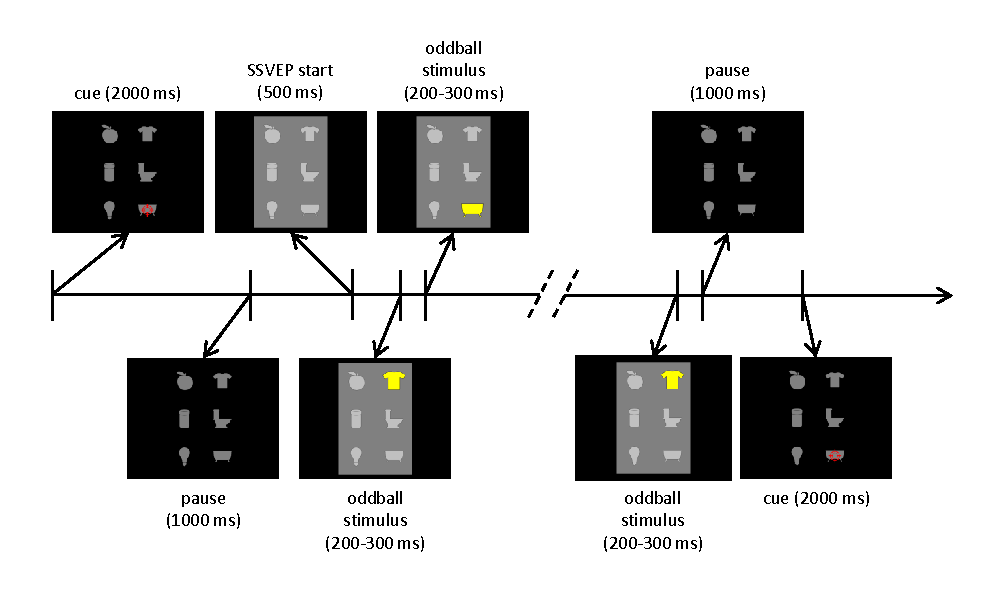
\includegraphics{pix/stimulationSequence}
\caption{stimulation sequence}
\label{fig:stimSeq}
\end{figure}

%===================================================================================================================
%                                             TABLES
%===================================================================================================================


%===================================================================================================================
%                                             FIGURES
%===================================================================================================================
\clearpage

%-------------------------------------------------------------------------------------------------------------------
% oddball pix
%-------------------------------------------------------------------------------------------------------------------
\begin{figure}[t]
\centering
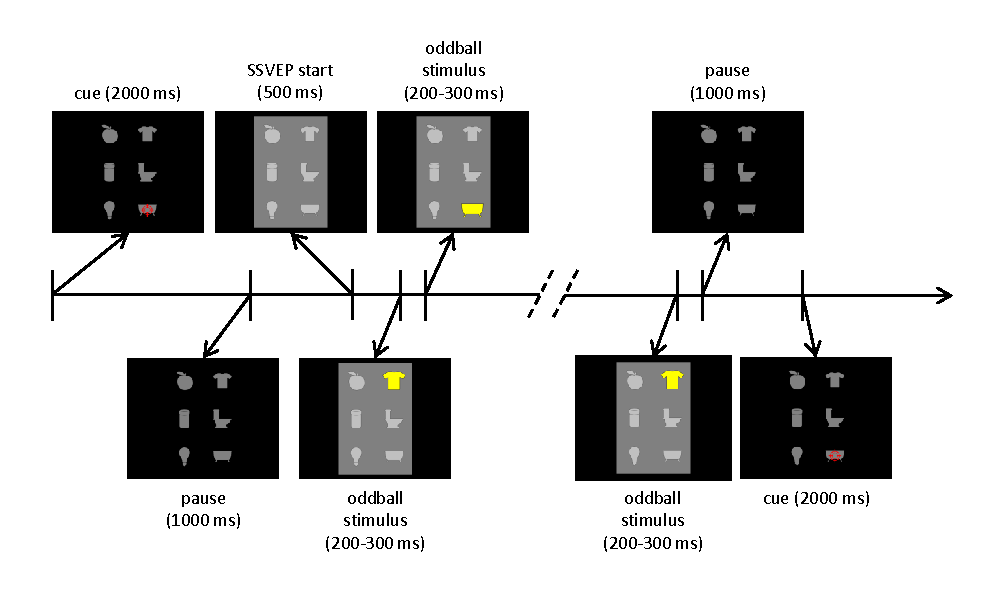
\includegraphics{pix/stimulationSequence}
\caption{stimulation sequence}
\label{fig:stimSeq}
\end{figure}

%\section{Acronyms}
%\begin{acronym}
%    \acro{SSVEP}{Steady-State Visually Evoked Potential}
%\end{acronym}

\end{document}
